`% !TeX root = ../defense.tex

\section{Data Preparation}
\frame{\sectionpage}


\begin{frame}{Corpus}
    \begin{enumerate}[<+->]\itemsep9pt
      \item Switchboard corpus . Originally recorded in 1991. 
      \item Audio recording of casual conversations between randomly chosen speakers.
      \item 2483 conversation, involving 520 speakers
      \item In our research we used the NXT version (S. Calhoun, 2010) of the corpus which contain 642 annotated conversations (XML)
    \end{enumerate}

\end{frame}{}


\begin{frame}{Preprocessing pipeline}
\begin{figure}[ht!]
\centering
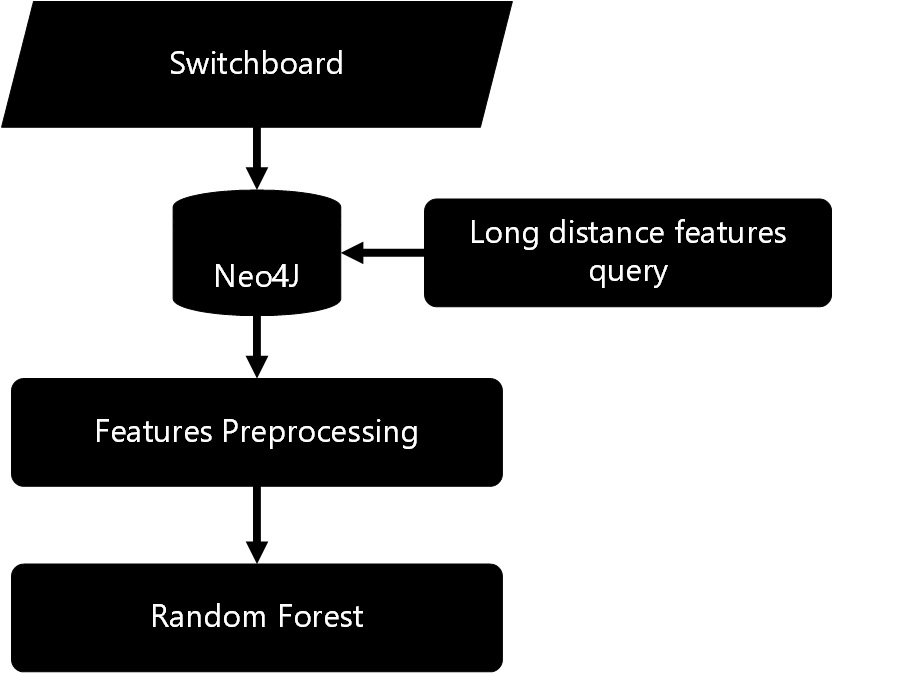
\includegraphics[width=20em]{../latex/pipeline.jpg}\vspace{-1em}
\end{figure}
\end{frame}


\begin{frame}{Conversation representation}
\begin{figure}[ht!]
\centering
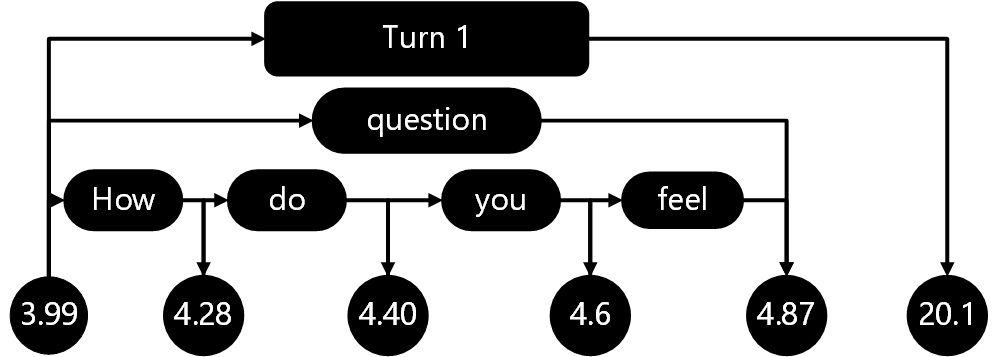
\includegraphics[width=30em]{../latex/graph5.jpg}\vspace{-1em}
\end{figure}
\end{frame}



\begin{frame}{Preprocessing}
 \begin{itemize}
    \item Removed 11 dialogue acts that were coded as other in switchboard.
    \item Reduce data sparsity by collapsing 65 dialog acts into 9.
    \item Performed using python-pandas.
  \end{itemize}

  \begin{table}
     \begin{center}
     \begin{tabular}{l | l}
    \hline
Switchboard dialog acts &  Dialog act classes  \\
    \hline
sd,h,bf      & statement   \\
sv,ad,sv@    & statement - opinion  \\
aa,aa\^r     & agree accept \\
\%.\%-,\%@   & abandon      \\
b,bh         & backchannel  \\
qy,qo,qh     & question     \\
no,ny,ng,arp & answer       \\
+            & +            \\
o@,+@        & NA           \\
  \hline
\end{tabular}
\end{center}\vspace{-0.5em}
\caption{Mapping from dialog act to dialog act class}
\label{tab:mapping}
\end{table}

\end{frame}{}


\section{Data Exploration}
\frame{\sectionpage}

\begin{frame}{Overview}
     \begin{enumerate}[<+->]\itemsep9pt
          \item Want to understand distribution of the input variables.
          \item Want to understand correlations between the input features and outcome (turn transition)
          \item Done using python pandas for data preparation and python seaborn for data visualization
      \end{enumerate}
\end{frame}


\begin{frame}{Dialog act relative count}
\begin{minipage}{0.8\textwidth}
\begin{figure}[H]
\centering
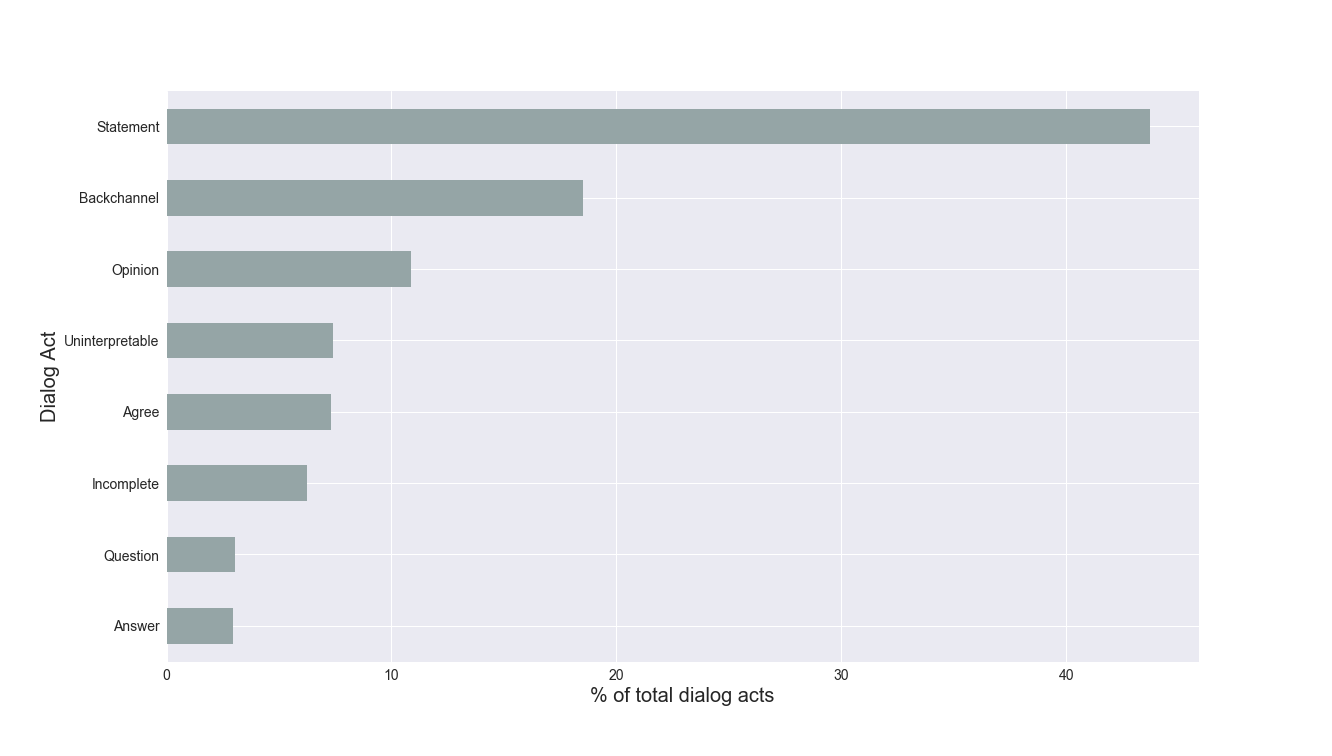
\includegraphics[width=30em]{../scikitlearn/figures/f1.png}
\end{figure}
\end{minipage}
\begin{minipage}{0.8\textwidth}
\begin{itemize}
\item Mainly Statements and Backchannels.
\item Representative of casual conversations.
\end{itemize}
\end{minipage}
\end{frame}

\begin{frame}{Turn Length Distribution}
\begin{minipage}{0.8\textwidth}
\begin{figure}[H]
\centering
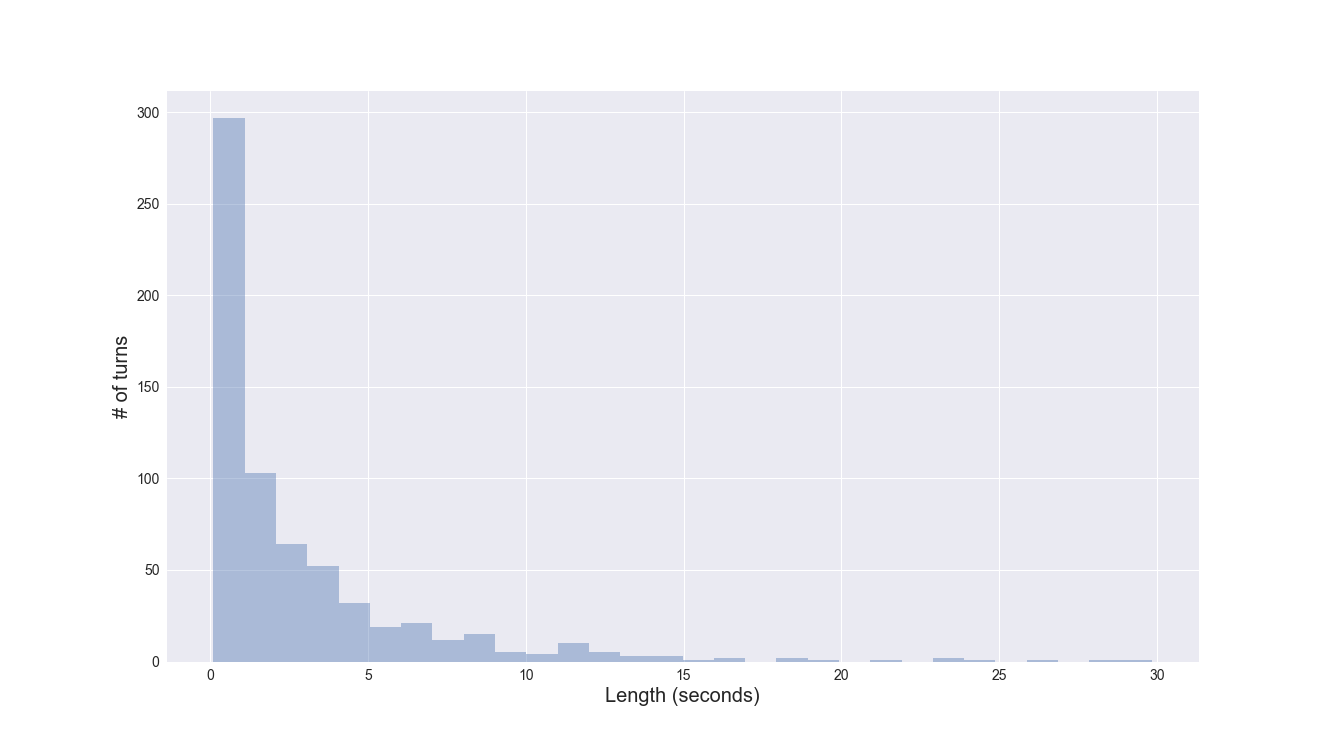
\includegraphics[width=30em]{../scikitlearn/figures/f10.png}\vspace{-1em}
\end{figure}
\end{minipage}
\begin{minipage}{0.8\textwidth}
\begin{itemize}
\item \small{Very skewed distribution}
\item \small{Long flat tail}
\end{itemize}
\end{minipage}
\end{frame}



\begin{frame}{Dialog act probability of turn change}
\begin{minipage}{0.8\textwidth}
\begin{figure}[H]
\centering
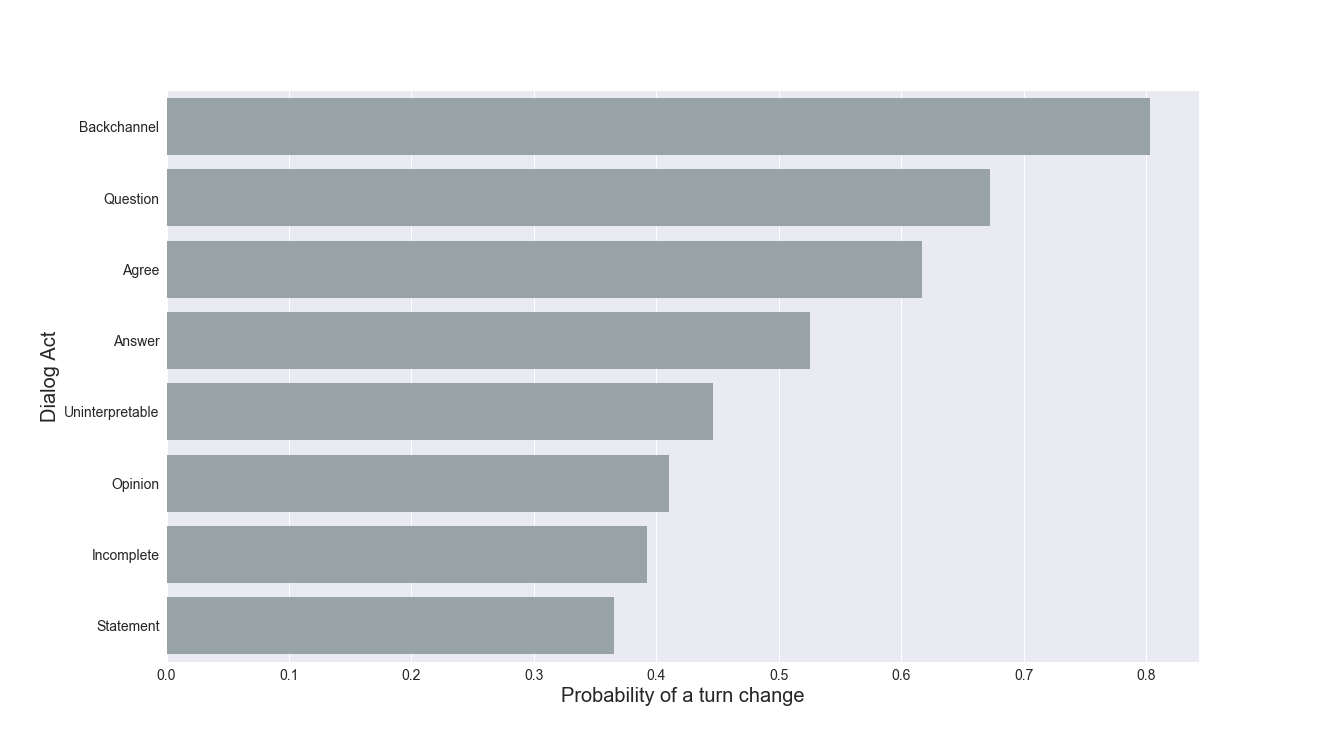
\includegraphics[width=30em]{../scikitlearn/figures/f2.png}\vspace{-1em}
\end{figure}
\end{minipage}
\begin{minipage}{0.8\textwidth}
\begin{itemize}
\item \small{Backchannels mostly leads to turn change (Explain the previous slide)}
\end{itemize}
\end{minipage}
\end{frame}



\begin{frame}{Relative Turn Length effect on probability of turn change}
\begin{minipage}{0.8\textwidth}
\begin{figure}[H]
\centering
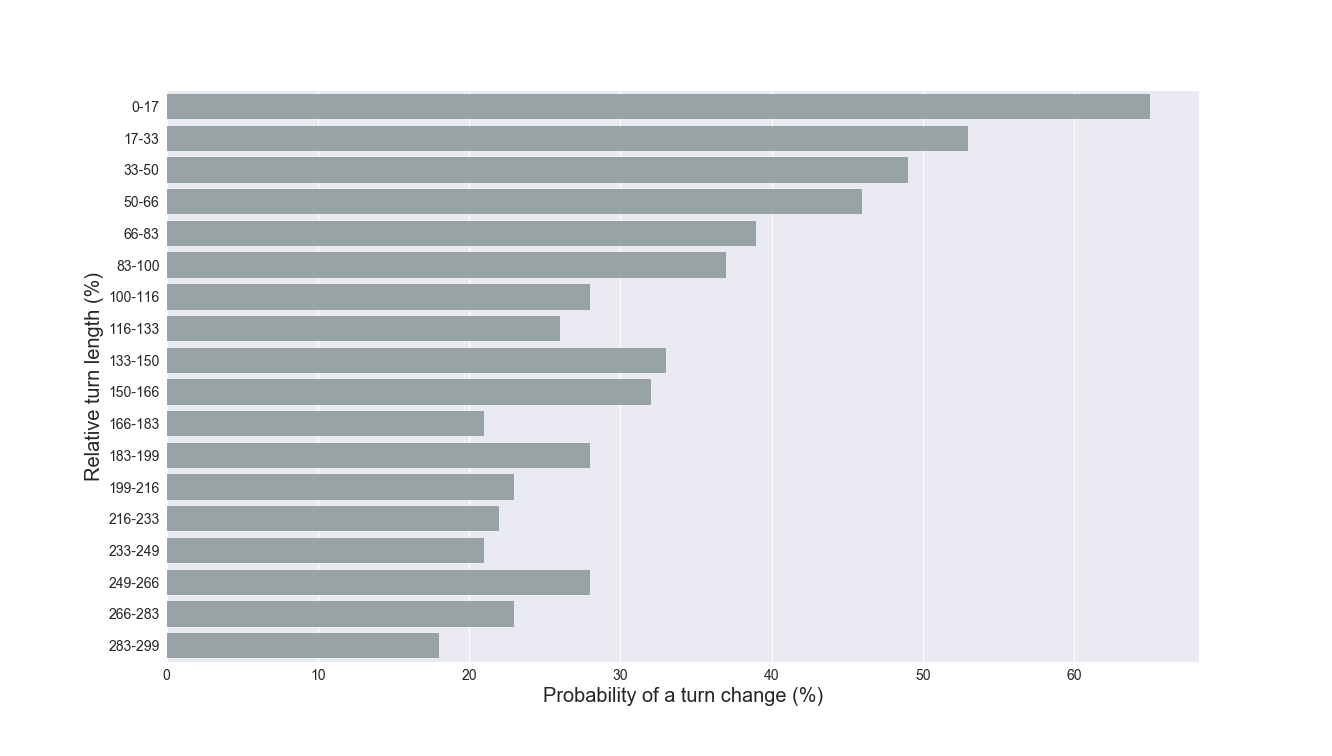
\includegraphics[width=36em]{../scikitlearn/figures/f5.png}\vspace{-1em}
\end{figure}
\end{minipage}
\begin{minipage}{0.8\textwidth}
\begin{itemize}
\item \small{Dialog act with small relative length lead to turn change.}
\item \small{As the speaker has the floor for more time, the speaker tends to hold it.}
\end{itemize}
\end{minipage}
\end{frame}

\begin{frame}{Relative Turn Control effect on probability of a turn change}
\begin{minipage}{0.8\textwidth}
\begin{figure}[H]
\centering
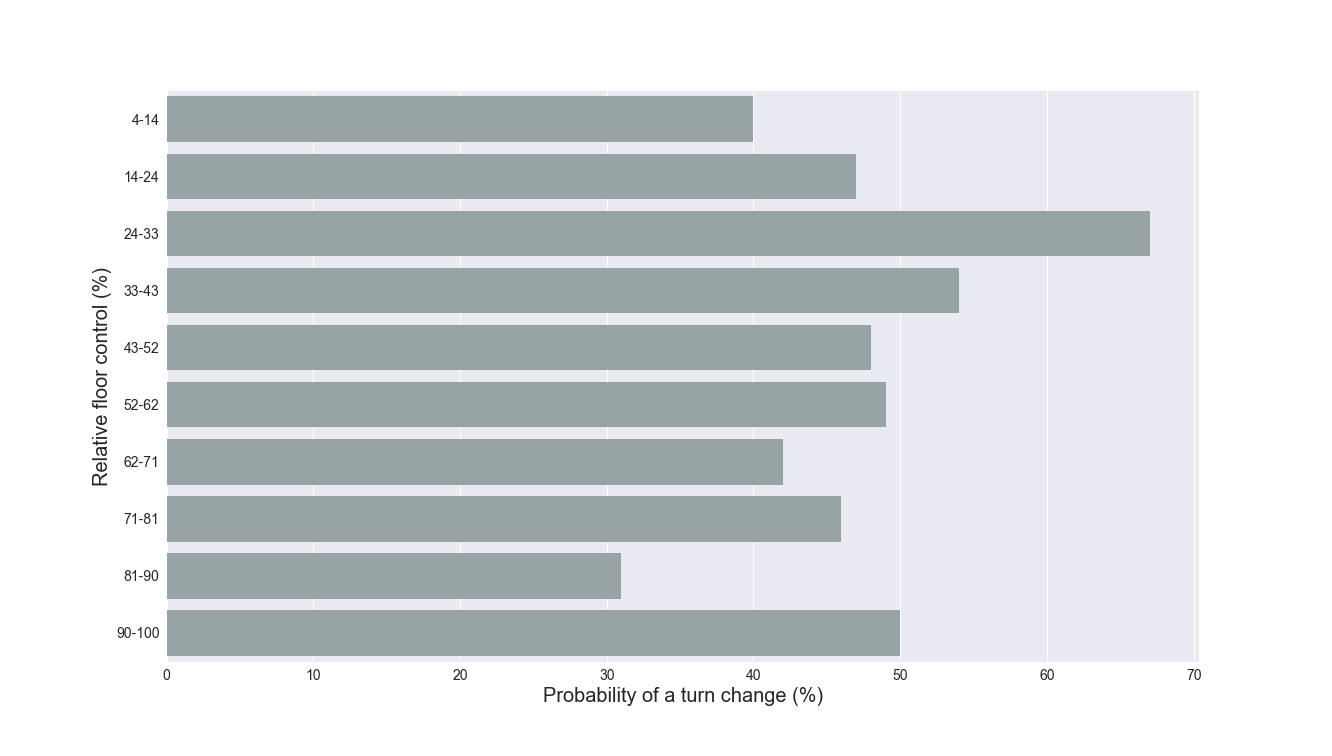
\includegraphics[width=30em]{../scikitlearn/figures/f6.png}\vspace{-1em}
\end{figure}
\end{minipage}
\begin{minipage}{0.8\textwidth}
\begin{itemize}
\item \small{High values of floor control correlate with the willingness of the current speaker to give up the floor.}
\end{itemize}
\end{minipage}
\end{frame}

\begin{frame}{Relative turn length for dialog act type}
\begin{minipage}{0.8\textwidth}
\begin{figure}[H]
\centering
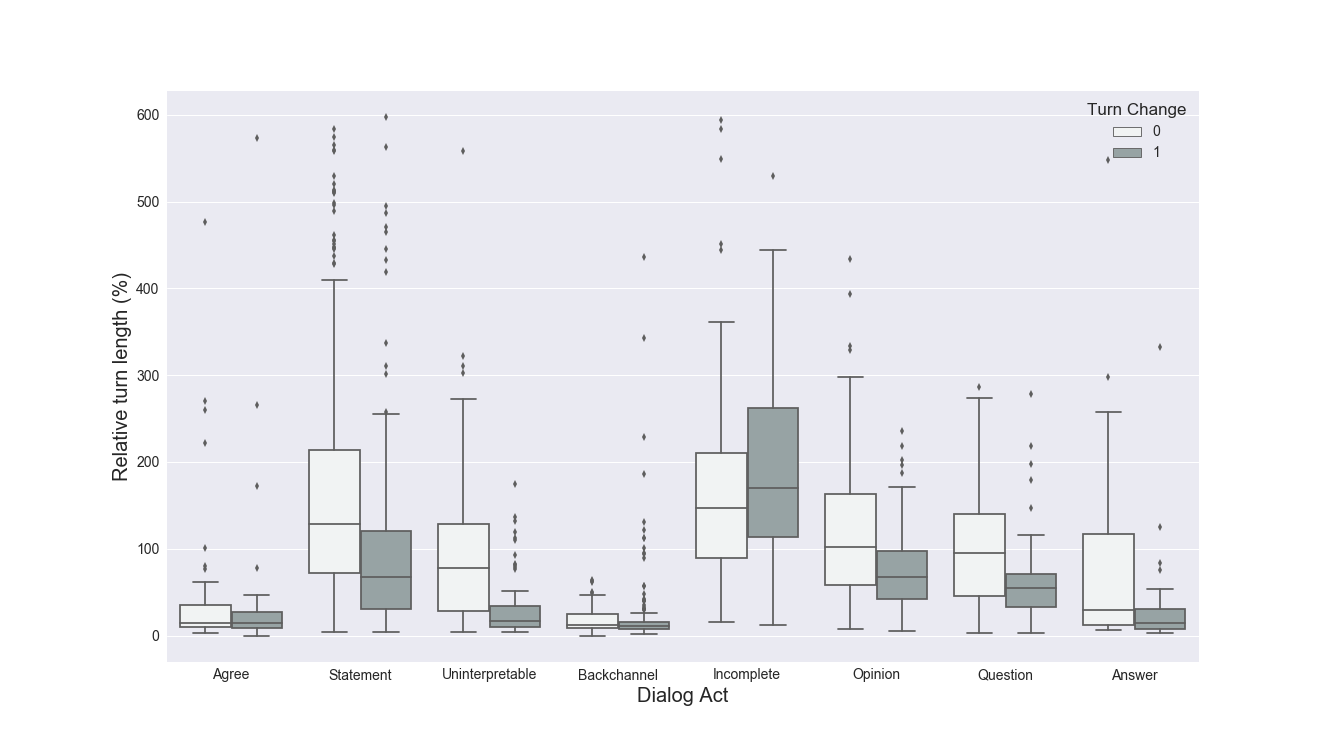
\includegraphics[width=30em]{../scikitlearn/figures/f3.png}\vspace{-1em}
\end{figure}
\end{minipage}
\begin{minipage}{0.8\textwidth}
\begin{itemize}
\item \small{The median relative turn length that led to a turn change is smaller than when it does not.}
\item \small{High RTL do not lead to turn change. Holds across dialog acts} 
\end{itemize}
\end{minipage}
\end{frame}


\begin{frame}{Relative floor control by dialog act}
\begin{minipage}{0.8\textwidth}
\begin{figure}[H]
\centering
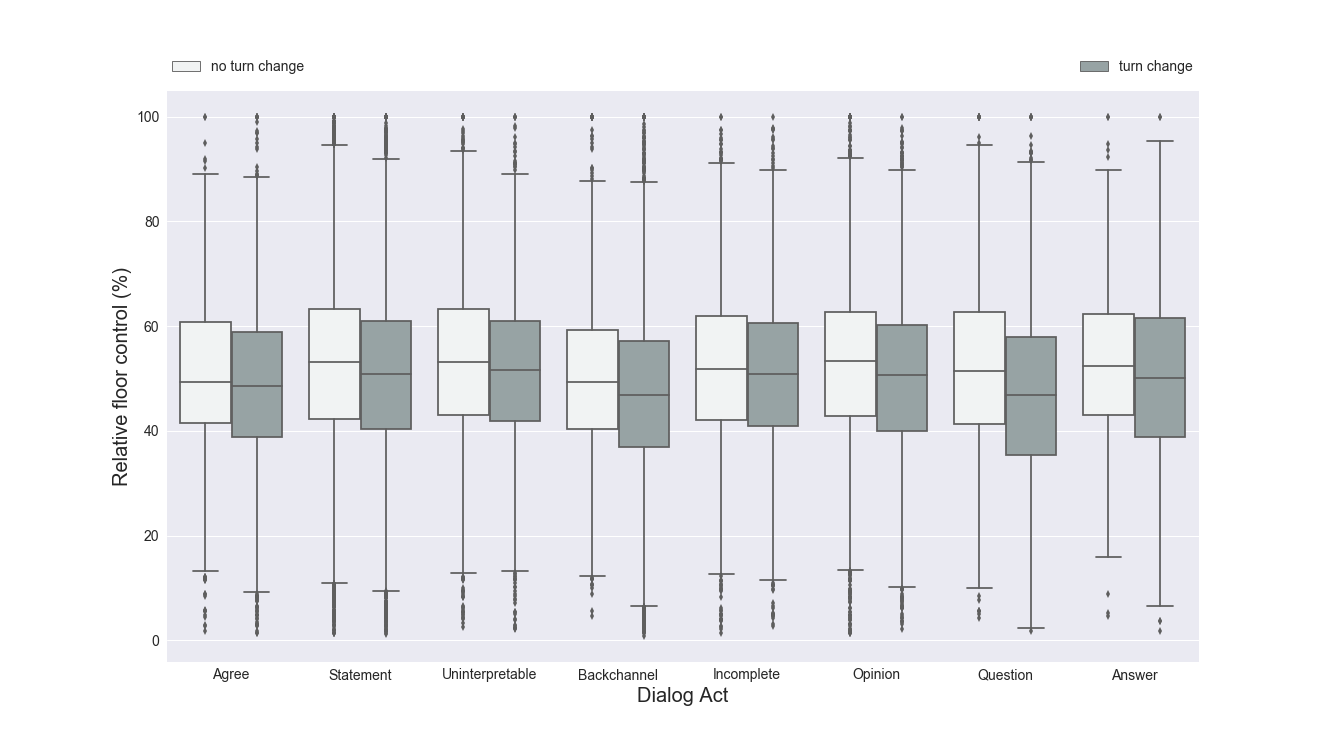
\includegraphics[width=30em]{../scikitlearn/figures/f4.png}\vspace{-1em}
\end{figure}
\end{minipage}
\begin{minipage}{0.8\textwidth}
\begin{itemize}
\item \small{The median is mainly 50\% across dialog acts}
\item \small{The median for relative floor control is slightly higher for each
dialogue act when it not followed by a turn change, than when it is}
\end{itemize}
\end{minipage}
\end{frame}


\begin{frame}{Exploration Summary}
 \begin{enumerate}[<+->]\itemsep9pt
          \item The chance of turn change is higher when the speaker has the floor for shorter than its average turn
          \item Contradict our initial assumption (that high RTL will lead to turn change)
          \item Possible explanation
                \begin{itemize}
                    \item for small relative turn length, this is due to short turn with single dialog act which is likely to be back channel or an answer, both of which have low relative
                     \item for high relative turn length, we attribute to the flat tail of turn length distribution - the chance that the current dialog act will lead to a turn change are smaller and smaller and hence the speaker will likely keep the floor
                \end{itemize}
  \end{enumerate}
\end{frame}

